\documentclass{article}
\usepackage[utf8]{inputenc}
\usepackage[UKenglish]{babel}
\usepackage[UKenglish]{isodate}
\usepackage{fullpage}
\usepackage{amsthm}
\usepackage{amsfonts}
\usepackage{amsmath}
\usepackage{mathtools}
\usepackage{hyperref}
\usepackage[capitalise]{cleveref}
\usepackage{bm}
\usepackage{booktabs}
\usepackage[table]{xcolor}
\usepackage{tikz}
\usepackage[backgroundcolor=lightgray]{todonotes}
\usepackage{complexity}
\usepackage{soul}
\usepackage[ruled,vlined]{algorithm2e}
\usepackage{subcaption}
\usepackage{multirow}

\newtheorem{theorem}{Theorem}
\newtheorem{observation}{Observation}
\newtheorem{lemma}{Lemma}
\newtheorem{proposition}{Proposition}
\newtheorem{corollary}{Corollary}
\newtheorem{conjecture}{Conjecture}
\theoremstyle{definition}
\newtheorem{definition}{Definition}
\newtheorem{example}{Example}
\theoremstyle{remark}
\newtheorem*{remark}{Remark}

\Crefname{property}{Property}{Properties}
\Crefname{condition}{Condition}{Conditions}
\creflabelformat{condition}{#2(#1)#3}

\DeclareMathOperator{\WMC}{WMC}
\DeclareMathOperator{\nWMC}{NWMC}
\DeclareMathOperator{\id}{id}
\DeclareMathOperator{\End}{End}
\DeclareMathOperator{\im}{im}

\usetikzlibrary{cd}
\usetikzlibrary{bayesnet}
\usetikzlibrary{calc}

\tikzset{
  Subset/.style={
    draw=none,
    every to/.append style={
      edge node={node [sloped, allow upside down, auto=false]{$\subset$}}}
  }
}

\title{Weighted Model Counting with Conditional Measures}
\author{Paulius Dilkas}

\begin{document}
\maketitle

\section{Introduction}

\begin{itemize}
\item The Main Narrative
  \begin{enumerate}
  \item When weights are defined on literals, the measure on the free BA is
    fully independent.
  \item This means that the BA itself must be larger (i.e., have additional
    `meaningless' literals) to turn any probability distribution into an
    independent one.
  \item We show how we can define conditional weights on literals, allowing us
    to encode any probability distribution into a Boolean algebra that's not
    necessarily independent and thus can be smaller.
  \item We demonstrate a specific example of this by presenting a new way to
    encode Bayesian networks into instances of WMC and adapting a WMC algorithm
    (ADDMC) to run on the new format.
  \item We show that this results in significantly faster inference.
  \item We show that our encoding results in asymptotically fewer literals and
    fewer ADDs, and thus a simpler problem.
  \item (Maybe) we experimentally demonstrate a phase transition based on the
    number of variables per ADD.
  \end{enumerate}
\item Potential criticism may be that this is a step backwards and doesn't allow
  us to use SAT-based techniques for probabilistic inference. However, they can
  still be used for the 'theory+query' part.
  \begin{itemize}
  \item Zero-probability weights and one-probability weights can be interpreted
    as logical clauses. This doesn't affect ADDMC but could be useful for other
    solvers.
  \end{itemize}
\item[F] What are the main claims, what are the main takeaways, intuitive [???]
  of theorems to follow. To do this, we appeal to algebraic constructions to
  define the main concepts for introducing measures on Boolean algebras.
\item
  Algorithms\footnote{\url{http://beyondnp.org/pages/solvers/model-counters-exact/}}
  \begin{itemize}
  \item ADDMC \cite{DBLP:conf/aaai/DudekPV20} (rediscovered the
    multiplicativity of BAs in different words) (with optimal settings)
  \item Cachet \cite{DBLP:conf/sat/SangBBKP04}
  \item c2d \cite{DBLP:conf/ecai/Darwiche04}
  \item d4 \cite{DBLP:conf/ijcai/LagniezM17} (closed source, boo!)
  \item miniC2D  \cite{DBLP:conf/ijcai/OztokD15}
  \end{itemize}
\item Notable previous/related work
  \begin{itemize}
  \item Hailperin's approach to probability logic
    \cite{DBLP:journals/ndjfl/Hailperin84}
  \item Nilsson's (somewhat successful) probabilistic logic
    \cite{DBLP:journals/ai/Nilsson86,DBLP:journals/ai/Nilsson93}
  \item Logical induction: a big paper with a good overview of previous attempts
    to assign probabilities to logical sentences in a sensible way
    \cite{DBLP:journals/eccc/GarrabrantBCST16}
  \item Measures on Boolean algebras
    \begin{itemize}
    \item On possibility and probability measures in finite Boolean algebras
      \cite{DBLP:journals/soco/CastineiraCT02}
    \item Representation of conditional probability measures
      \cite{krauss1968representation}
    \end{itemize}
  \end{itemize}
\item Intuitively, a measure is just like a probability, except it's in
  $\mathbb{R}_{\ge 0}$ instead of $[0, 1]$.
\end{itemize}

\section{Preliminaries}

\begin{itemize}
\item Make up my mind about $a, b$ vs. $x, y$ and stick to it (maybe $x, y$?).
\item Terminology: `with generating set $S$' $\to$ `over $S$'.
\item Notation: if $L$ denotes literals, then it doesn't denote a generating
  set. Literals should be $U$.
\item Describe the parallel between BAs and powersets.
\item Describe \cref{tbl:notation_example} as an example. We will use
  set-theoretic notation for $2^U$ and Boolean-algebraic notation for $2^{2^U}$
  (except for atoms).
\end{itemize}

\begin{table}
  \caption{(in the same order)}
  \label{tbl:notation_example}
  \centering
  \begin{tabular}{lcc}
    \toprule
    & Set-theoretic notation & Boolean-algebraic notation \\
    \midrule
    Atoms (elements of $U$) & $a, b$ & $a, b$ \\
    \rowcolor{gray!10} Models (elements of $2^U$) & $\emptyset, \{a\}, \{b\}, \{a, b\}$ & $\neg a \land \neg b, a \land \neg b, \neg a \land b, a \land b$ \\
    & $\{ \emptyset, \{a\}, \{b\}, \{a, b\} \}$ & $\top$ \\
    & $\{ \emptyset, \{a\}, \{b\} \}, \{ \emptyset, \{a\}, \{a, b\} \}$ & $\neg a \lor \neg b, a \to b$ \\
    & $\{ \emptyset, \{b\}, \{a, b\} \}, \{ \{a\}, \{b\}, \{a, b\} \}$ & $b \to a, a \lor b$ \\
    & $\{\emptyset, \{a\}\}, \{\emptyset, \{b\}\}, \{\emptyset, \{a, b\}\}$ & $\neg b, \neg a, a \leftrightarrow b$ \\
    & $\{\{a\}, \{b\}\}, \{\{a\}, \{a, b\}\}, \{\{b\}, \{a, b\}\}$ & $(a \land \neg b) \lor (b \land \neg a), a, b$ \\
    & $\{\emptyset\}, \{\{a\}\}, \{\{b\}\}, \{\{a, b\}\}$ & $\neg a \land \neg b, a \land \neg b, \neg a \land b, a \land b$ \\
    \multirow{-7}{*}{Formulas (elements of $2^{2^U}$)} & $\emptyset$ & $\bot$ \\
    \bottomrule
  \end{tabular}
\end{table}

Consider the Boolean algebra $(2^{2^U}, \land, \lor, \neg, \bot, \top)$. A
partial order $\le$ on $2^{2^U}$ is defined by $a \le b$ if $a = b \land a$ (or,
equivalently, $a \lor b = b$) for all $a, b \in 2^{2^U}$.

\begin{definition}[\cite{DBLP:books/daglib/0090259,levasseur2012applied}]
  An element $a \ne 0$ of $2^{2^U}$ is an \emph{atom} if, for all $x \in
  2^{2^U}$, either $x \land a = a$ or $x \land a = 0$. Equivalently, $a \ne 0$
  is an atom if there is no $x \in \mathbf{B}$ such that $0 < x < a$.
  Equivalently, $a \ne 0$ is an atom if $|a| = 1$, i.e., $a = \{ u \}$ for some
  $u \in 2^U$ (this is how we will denote atoms in the remainder of the paper).
  Note that atoms in Boolean algebras correspond to models.
\end{definition}

\begin{lemma}[\cite{givant2008introduction}] \label{thm:representation}
  The following are equivalent:
  \begin{itemize}
  \item $\mathbf{B}$ is atomic.
  \item For any $x \in \mathbf{B}$, $x = \bigvee_{\text{atoms } a \le x} a$.
  \item $1$ is the supremum of all atoms.
  \end{itemize}
\end{lemma}

\begin{definition}[\cite{gaifman1964concerning,DBLP:books/daglib/0090259}] \label{def:measure}
  A \emph{measure} on $\mathbf{B}$ is a function $m\colon
  \mathbf{B} \to \mathbb{R}_{\ge 0}$ such that:
  \begin{itemize}
  \item $m(0) = 0$;
  \item $m(a \lor b) = m(a) + m(b)$ for all $a, b \in \mathbf{B}$ whenever $a
    \land b = 0$.
  \end{itemize}
  If $m(1) = 1$, we call $m$ a \emph{probability measure}. Also, if $m(x) > 0$
  for all $x \ne 0$, then $m$ is \emph{strictly positive}.
\end{definition}

\begin{lemma}[\cite{sikorski1969boolean}] \label{lemma:order}
  For any $a, b \in \mathbf{B}$, $a \le b$ if and only if $a \land \neg b = 0$.
\end{lemma}

\begin{lemma}[\cite{givant2008introduction}] \label{lemma:measure_and_order}
  Let $m\colon \mathbf{B} \to \mathbb{R}_{\ge 0}$ be a measure. Then for all $a,
  b \in \mathbf{B}$, if $a \le b$, then $m(a) \le m(b)$.
\end{lemma}

\subsection{The Space of Functions on Boolean Algebras}

\begin{definition}[Operations on functions]
  Let $A\colon 2^X \to \mathbb{R}_{\ge 0}$ and $B\colon 2^Y \to \mathbb{R}_{\ge
    0}$ be Boolean functions, $\alpha \in \mathbb{R}_{\ge 0}$, and $x \in X$. We
  define the following operations:
  \begin{description}
  \item[Addition:] $A+B$ is a function $A+B\colon 2^{X \cup Y} \to
    \mathbb{R}_{\ge 0}$ such that
    \[
      (A+B)(\tau) = A(\tau \cap X) + B(\tau \cap Y)
    \]
    for all $\tau \in 2^{X \cup Y}$.
  \item[Inverse:] $\overline{A}$ is a function $\overline{A}\colon 2^X \to
    \mathbb{R}_{\ge 0}$ such that
    \[
      \overline{A}(\tau) = 1 - A(\tau)
    \]
    for all $\tau \in 2^X$.
  \item[Multiplication:] $A \cdot B$ is a function $A \cdot B\colon 2^{X \cup Y}
    \to \mathbb{R}_{\ge 0}$ such that
    \[
      (A \cdot B)(\tau) = A(\tau \cap X) \cdot B(\tau \cap Y)
    \]
    for all $\tau \in 2^{X \cup Y}$.
  \item[Scalar multiplication:] $\alpha A$ is a function $\alpha A\colon 2^X \to
    \mathbb{R}_{\ge 0}$ such that
    \[
      (\alpha A)(\tau) = \alpha \cdot A(\tau)
    \]
    for all $\tau \in 2^X$.
  \item[Projection:] $\exists_xA$ is a function $\exists_xA\colon 2^{X \setminus
      \{ x \}} \to \mathbb{R}_{\ge 0}$ such that
    \[
      (\exists_xA)(\tau) = A(\tau) + A(\tau \cup \{ x \})
    \]
    for all $\tau \in 2^{X \setminus \{x \}}$.
  \end{description}
\end{definition}

\begin{observation}
  Let $\mathcal{V} = \{ A\colon 2^X \to \mathbb{R}_{\ge 0} \mid X \subseteq U
  \}$. Then $\mathcal{V}$ is a semi-vector space with three additional
  operations: inverse, (non-scalar) multiplication, and projection.
  Specifically, note that both addition and multiplication are both associative
  and commutative.
\end{observation}

\begin{definition}[Special functions]
  \phantom{}
  \begin{itemize}
  \item unit $1\colon 2^\emptyset \to \mathbb{R}_{\ge 0}$, $1(\tau) = 1$.
  \item zero $0\colon 2^\emptyset \to \mathbb{R}_{\ge 0}$, $0(\tau) = 0$.
  \item constant $[a]\colon 2^{\{a\}} \to \mathbb{R}_{\ge 0}$,
    \[
      [a](\tau) =
      \begin{cases}
        1 & \text{if } a \in \tau \\
        0 & \text{if } a \not\in \tau.
      \end{cases}
    \]
  \end{itemize}
\end{definition}

\begin{remark}
  For any function $A\colon 2^X \to \mathbb{R}_{\ge 0}$, $A + \overline{A} = 1$.
\end{remark}

Henceforth, for any function $A\colon 2^X \to \mathbb{R}_{\ge 0}$ and any set
$\tau$, we will write $A(\tau)$ to mean $A(\tau \cap X)$.

\section{Weighted Model Counting as a Measure}

\begin{itemize}
\item[F2] Explain with examples: models $=$ elements [atoms] of algebra.
\item Be careful about mentioning ideals and quotients.
\end{itemize}

\begin{definition} \label{def:wmc}
  Let $U$ be an arbitrary set. Then
  \begin{itemize}
  \item a \emph{measure} is a function $M\colon 2^{2^U} \to \mathbb{R}_{\ge 0}$,
  \item a \emph{weight function} is a function $W\colon 2^U \to \mathbb{R}_{\ge
      0}$.
  \item a weight function is \emph{factored} if $W = \prod_{x \in U} W_x$ for
    some functions $W_x\colon 2^{\{x\}} \to \mathbb{R}_{\ge 0}$.
  \item every weight function induces a measure:
    \[
      M_W(x) = \begin{cases}
        0 & \text{if } x = \bot \\
        W(u) & \text{if } x = \{ u \} \\
        \sum_{\{u\} \le x} W(u) & \text{otherwise.}
      \end{cases}
    \]
    The process of calculating the value of $M_W(x)$ for some $x \in 2^{2^U}$
    with a given definition of $W$ is known as \emph{weighted model counting}.
  \item A measure $M\colon 2^{2^U} \to \mathbb{R}_{\ge 0}$ is
    \emph{factorable} if there exists a factored weight function $W\colon 2^U
    \to \mathbb{R}_{\ge 0}$ that induces $M$.
  \end{itemize}
\end{definition}

\begin{example} \label{example:construction}
  Let $\mathcal{L}$ be a propositional logic with $p$ and $q$ as its only atoms.
  Then $L = \{ p, q, \neg p, \neg q \}$ is its set of literals. Let $w : L \to
  \mathbb{R}_{\ge 0}$ be the \emph{weight function} defined by
  \begin{align*}
    w(p) = 0.3, \\
    w(\neg p) = 0.7, \\
    w(q) = 0.2, \\
    w(\neg q) = 0.8.
  \end{align*}
  Let $\Delta$ be a theory in $\mathcal{L}$ with a sole axiom $p$. Then
  $\Delta$ has two models, i.e., $\{ p, q \}$ and $\{ p, \neg q \}$. The
  \emph{weighted model count} (WMC) \cite{DBLP:journals/ai/ChaviraD08} of $\Delta$ is
  then
  \[
    \sum_{\omega \models \Delta} \prod_{\omega \models l} w(l) =
    w(p)w(q) + w(p)w(\neg q) = 0.3.
  \]

  The corresponding BA $B(\Delta)$ can then be constructed as a
  Lindenbaum-Tarski algebra. Alternatively, one can first construct the free
  BA generated by the set $\{ p, q \}$ and then take a quotient with respect to
  either the filter generated by $p$ or the ideal\footnote{More details on these
    concepts can be found in many books on BAs
    \cite{givant2008introduction,koppelberg1989handbook}.} generated by $\neg
  p$.

  Each element of $B(\mathcal{L})$ can also be seen as a subset of the set of
  all models of $\mathcal{L}$, with $0$ representing $\emptyset$, $1$
  representing the set of all (four) models, each atom representing a single
  model, and each edge going upward representing a subset relation. Thus,
  the Boolean-algebraic way of calculating the WMC of $\Delta$ consists of:
  \begin{enumerate}
  \item Identifying an element $a \in B(\mathcal{L})$ that corresponds to
    $\Delta$.
  \item Finding all atoms of $B(\mathcal{L})$ that are `dominated' by $a$
    according to the partial order.
  \item Using $w$ to calculate the weight of each such atom.
  \item Adding the weights of these atoms.
  \end{enumerate}
  This motivates the following definition of WMC generalised to BAs.
\end{example}
\todo[inline,caption={}]{
  \begin{itemize}
  \item Why is Step 1 always possible?
  \item Clarify what $B(L)$ means and whether $B(\Delta)$ is even necessary.
  \item Find a reference for the set/subset thing.
  \end{itemize}
}

Given a theory $\Delta$ in a logic $\mathcal{L}$, the usual way of using WMC to
compute the probability of a query $q$ is
\cite{DBLP:conf/uai/Belle17,DBLP:conf/aaai/SangBK05}
\[
  \Pr_{\Delta, w}(q) = \frac{\WMC_w(\Delta \land q)}{\WMC_w(\Delta)}.
\]
In our algebraic formulation, this can be computed in two different ways:
\begin{itemize}
\item as $\frac{\WMC_w(\Delta \land q)}{\WMC_w(\Delta)}$ in $B(\mathcal{L})$,
\item and as $\nWMC_w([q])$ in $B(\Delta)$.
\end{itemize}
But how does the measure defined on $B(\mathcal{L})$ transfer to $B(\Delta)$?

\section{Limitations of Factorable Measures}

\begin{itemize}
\item[F] Give a concrete example of something impossible to represent using WMC.
\item[F] Can you say something here about factorized vs non-factorized
  weight function definitions? That is, factorized is when $w$ maps literals to
  $R_{\ge 0}$, non-factorized is when $w$ maps models to $R_{\ge 0}$ and
  \begin{itemize}
  \item come up with nice example when non-factorized weights are intuitive;
  \item clarify that the factorized definition have is w.r.t. models, in case some
    one gets confused. [It doesn't have to be, if the BA is not free---P.]
  \end{itemize}
\end{itemize}

\begin{lemma} \label{lemma:before_theorem}
  For any measure $M\colon 2^{2^U} \to \mathbb{R}_{\ge 0}$ and elements $a, b
  \in 2^{2^U}$,
  \begin{equation} \label{eq:to_prove}
    M(a \land b) = M(a)M(b)
  \end{equation}
  if and only if
  \begin{equation} \label{eq:to_prove2}
    M(a \land b) \cdot M(\neg a \land \neg b) = M(a \land \neg b)
    \cdot M(\neg a \land b).
  \end{equation}
\end{lemma}
\begin{proof}
  First, note that $a = (a \land b) \lor (a \land \neg b)$ and $(a \land b)
  \land (a \land \neg b) = 0$, so, by properties of a measure,
  \begin{equation} \label{eq:temp}
    M(a) = M(a \land b) + M(a \land \neg b).
  \end{equation}
  Applying \cref{eq:temp} and the equivalent expression for $M(b)$ allows us
  to rewrite \cref{eq:to_prove} as
  \[
    M(a \land b) = [M(a \land b) + M(a \land \neg b)][M(a \land b) + M(\neg a
    \land b)]
  \]
  which is equivalent to
  \begin{equation} \label{eq:temp6}
    M(a \land b)[1 - M(a \land b) - M(a \land \neg b) - M(\neg a \land b)] = M(a
    \land \neg b)M(\neg a \land b).
  \end{equation}
  Since $a \land b$, $a \land \neg b$, $\neg a \land b$, $\neg a \land \neg b$
  are pairwise disjoint and their supremum is $1$,
  \[
    M(a \land b) + M(a \land \neg b) + M(\neg a \land b) + M(\neg a \land \neg
    b) = 1,
  \]
  and this allows us to rewrite \cref{eq:temp6} into \cref{eq:to_prove2}. As all
  transformations are invertible, the two expressions are equivalent.
\end{proof}

\todo[inline]{This theorem needs a special case for zero weights.}
\begin{theorem}
  A measure $M\colon 2^{2^U} \to \mathbb{R}_{\ge 0}$ is factorable if and only
  if
  \begin{equation} \label{eq:wmccondition}
  M(u \land v) = M(u)M(v)
  \end{equation}
  for all distinct $u, v \in U \cup \{ \neg w \mid w \in U \}$ such that $u \ne
  \neg v$.
\end{theorem}
\begin{proof}
  ($\Leftarrow$) For each $x \in U$, let $W_x\colon 2^{\{x\}} \to
  \mathbb{R}_{\ge 0}$ be defined by $W_x(\{ x \}) = M(x)$ and $W_x(\emptyset) =
  M(\neg x)$. Let $M_W$ be the measure induced by
  \[
    W = \prod_{x \in U} W_x.
  \]
  We will show that $M = M_W$. First, note that $M_w(\bot) = 0 = M(\bot)$ by the
  definitions of both $M_w$ and $M$. Second, let
  \begin{equation} \label{eq:def_of_a}
    a = \bigwedge_{u \in U} a_u
  \end{equation}
  be an atom in $2^{2^U}$ such that $a_u \in \{ u, \neg u \}$ for all $u \in U$.
  Then
  \[
    M_W(a) = \prod_{u \in U} W_u(a_u) = \prod_{u \in U} M(a_u) = M
    \left(\bigwedge_{u \in U} a_u \right) = M(a)
  \] % TODO: by what?
  by \cref{def:wmc,eq:wmccondition,eq:def_of_a}. Finally, note that if $M_W$ and
  $M$ agree on all atoms, then they must also agree on all other non-zero
  elements of the Boolean algebra.

  ($\Rightarrow$) For the other direction, we are given a factored weight
  function
  \[
    W = \prod_{x \in U} W_x,
  \]
  and we want to show that its induced measure $M_W$ satisfies
  \cref{eq:wmccondition}. Let $k_u, k_v \in U \cup \{ \neg w \mid w \in U \}$ be
  such that $k_u \in \{ u, \neg u \}$, $k_v \in \{ v, \neg v \}$, and $u \ne v$.
  We then want to show that
  \begin{equation} \label{eq:to_prove3}
    M_W(k_u \land k_v) = M_W(k_u)M_W(k_v)
  \end{equation}
  which is equivalent to
  \begin{equation} \label{eq:to_prove4}
    M_W(k_u \land k_v) \cdot M_W(\neg k_u \land \neg k_v) = M_W(k_u \land \neg k_v) \cdot M_w(\neg k_u \land k_v)
  \end{equation}
  by \cref{lemma:before_theorem}. Then
  \begin{align*}
    M_W(k_u \land k_v) &= \sum_{\{a\} \le k_u \land k_v} W(a) = \sum_{\{a\} \le k_u \land k_v} \prod_{x \in U} W_x(a) \\
                        &= \sum_{\{a\} \le k_u \land k_v} W_u(a_u)W_v(a_v) \prod_{x \in U \setminus \{ u, v \}} W_x(a) = \sum_{\{a\} \le k_u \land k_v} W_u(k_u)W_v(k_v) \prod_{x \in U \setminus \{ u, v \}} W_x(a) \\
    &= W_u(k_u)W_v(k_v) \sum_{\{a\} \le k_u \land k_v} \prod_{x \in U \setminus \{ u, v \}} W_x(a) = W_u(k_u)W_v(k_v)C,
  \end{align*}
  where $C$ denotes the part of $M_W(k_u \land k_v)$ that will be the same for
  $M_W(\neg k_u \land k_v)$, $M_W(k_u \land \neg k_v)$, and $M_W(\neg k_u \land
  \neg k_v)$ as well. But then \cref{eq:to_prove4} becomes
  \[
    W_u(k_u)W_v(k_v)W_u(\neg k_u)W_v(\neg k_v)C^2 = W_u(k_u)W_v(\neg
    k_v)W_u(\neg k_u)W_v(k_v)C^2
  \]
  which is trivially true.
\end{proof}

Given this requirement for independence, a well-known way to represent
probability distributions that do not consist entirely of independent variables
is by adding more literals \cite{DBLP:journals/ai/ChaviraD08}, i.e., extending
the set $L$ covered by the WMC weight function $w\colon L \to \mathbb{R}_{\ge
  0}$. More precisely, we are given the left-hand column in
\[
  \begin{tikzcd}
    \textcolor{red}{\mathbb{R}_{\ge 0}} & & \\
    \textcolor{red}{\mathbf{B}} \arrow[red]{u}{m} \ar[r,hookrightarrow,"\iota"]
    & \mathbf{B'} \arrow{lu}[swap]{m'} & \\
    \textcolor{red}{L} \ar[u,red,hookrightarrow] \ar[r,hookrightarrow] & L'
    \ar[u,hookrightarrow] \arrow{r}{w} & \mathbb{R}_{\ge 0}
  \end{tikzcd}
\]
and construct the remaining part in such a way that the triangle commutes.

\todo[inline]{Must quotient the BA w.r.t. some rules.}

\section{Previous Work}

\subsection{Bayesian Network Encodings}

\begin{itemize}
\item \texttt{cd05} relaxes the encoding so much that extra models become
  possible. They are supposed to be filtered out by the algorithm, but mine
  can't do that because it doesn't deal with models. Same for \texttt{cd06}
  because it's based on \texttt{cd05}.
\item \texttt{sbk05} uses my trick with dividing probabilities. That could
  explain small inaccuracies in its answers.
\item Encodings:
  \begin{itemize}
  \item \texttt{d02} \cite{DBLP:conf/kr/Darwiche02}
  \item \texttt{sbk05} \cite{DBLP:conf/aaai/SangBK05}
  \item \texttt{cd05} \cite{DBLP:conf/ijcai/ChaviraD05}
  \item \texttt{cd06} \cite{DBLP:conf/sat/ChaviraD06} (supposed to be the best)
  \item \texttt{db20} (mine)
  \end{itemize}
\end{itemize}

\subsection{Algebraic Decision Diagrams and ADDMC}

References
\begin{itemize}
\item ADDs \cite{DBLP:journals/fmsd/BaharFGHMPS97}
\item background reading
  \begin{itemize}
  \item Compiling Bayesian Networks Using Variable Elimination (Chavira and
    Darwiche) \cite{DBLP:conf/ijcai/ChaviraD07}
  \item On the Relationship between Sum-Product Networks and Bayesian Networks
    (Zhao et al.) \cite{DBLP:conf/icml/ZhaoMP15}
  \end{itemize}
\end{itemize}

\section{Encoding Bayesian Networks Using Conditional Weights}

\begin{itemize}

\item We assume that all variables in the Bayesian network have at least two
  values.
\item Have an example of how the ADDs function in this situation. If not for the
  paper, then at least for slides. Use the framework to check its correctness.
\item The function $\phi$ created by the algorithm can be seen as a measure on
  the BA $2^{2^U}$.
\item We extend the Gaifman graph to add edges when two variables occur in the
  same CPT (e.g., including the edge from $A$ to $B$ when the CPT is $\Pr(A \mid
  B)$).
\end{itemize}

Let $V$ denote the set of random variables in a Bayesian network. For any random
variable $X \in V$, let $\mathrm{pa}(X)$ denote the set of parents of $X$ and
$\im X$ denote the set of possible values.

\begin{definition}[Indicator variables]
  Let $X \in V$ be a random variable. If $X$ is binary (i.e., $|\im X| = 2$), we
  can arbitrary identify one of the values as $1$ and the other one as $0$ (i.e,
  $\im X \cong \{ 0, 1 \}$). Then $X$ can be represented by a single
  \emph{indicator variable} $\lambda_{X=1}$. For notational simplicity, for any
  set $S$, whenever we write $\lambda_{X=0} \in S$ or $S = \{ \lambda_{X=0},
  \dots \}$, we actually mean $\lambda_{X=1} \not\in S$,

  On the other hand, if $X$ is not binary, we represent $X$ with $|\im X|$
  indicator variables, one for each value. We let
  \[
    E(X) = \begin{cases}
      \{ \lambda_{X=1} \} & \text{if } |\im X| = 2 \\
      \{ \lambda_{X=x} \mid x \in \im X \} & \text{otherwise.}
    \end{cases}
  \]
  denote the set of indicator variables for $X$ and
  \[
    E^*(X) = E(X) \cup \bigcup_{Y \in \mathrm{pa}(X)} E(Y).
  \]
  denote the set of indicator variables for $X$ and its parents in the Bayesian
  network. Finally, let
  \[
    U = \bigcup_{X \in V} E(X)
  \]
  denote the set of all indicator variables for all random variables in the
  Bayesian network.
\end{definition}

\begin{algorithm}
  $\phi \gets 1$\;
  \For{$X \in V$}{
    \textit{let} $\mathrm{pa}(X) = \{ Y_1, \dots, Y_n \}$\;
    $\mathrm{CPT}_X \gets 0$\;
    \eIf{$|\im X| = 2$}{
      \For{$(y_1, \dots, y_n) \in \prod_{i = 1}^n \im Y_i$}{
        $p_1 \gets \Pr(X = 1 \mid Y_1 = y_1, \dots, Y_n = y_n)$\;
        $p_0 \gets \Pr(X \ne 1 \mid Y_1 = y_1, \dots, Y_n = y_n)$\;
        $\mathrm{CPT}_X \gets \mathrm{CPT}_X + p_1[\lambda_{X=1}] \cdot
        \prod_{i=1}^n [\lambda_{Y_i=y_i}] + p_0 \overline{[\lambda_{X=1}]} \cdot
        \prod_{i=1}^n [\lambda_{Y_i=y_i}]$\;
      }
    }{
      \textit{let} $\im X = \{ x_1, \dots, x_m \}$\;
      \For{$x \in \im X$ {\rm \textbf{and}} $(y_1, \dots, y_n) \in \prod_{i =
          1}^n \im Y_i$}{
        $p_x \gets \Pr(X = x \mid Y_1 = y_1, \dots, Y_n = y_n)$\;
        $\mathrm{CPT}_X \gets \mathrm{CPT}_X + p_x[\lambda_{X=x}] \cdot
        \prod_{i=1}^n [\lambda_{Y_i=y_i}] + \overline{[\lambda_{X=1}]} \cdot
        \prod_{i=1}^n [\lambda_{Y_i=y_i}]$\;
      }
      $\mathrm{CPT}_X \gets \mathrm{CPT}_X \cdot \left( \sum_{i=1}^m [\lambda_{X
          = x_i}] \right) \cdot \prod_{i=1}^m \prod_{j=i+1}^m
      (\overline{[\lambda_{X = x_i}]} + \overline{[\lambda_{X = x_j}]})$\;
    }
    $\phi \gets \phi \cdot \mathrm{CPT}_X$\;
  }
  \Return{$\phi$}\;
\end{algorithm}

\begin{lemma} \label{lemma:cpt}
  Let $X \in V$ be a random variable with parents $\mathrm{pa}(X) = \{ Y_1,
  \dots, Y_n \}$. Then $\mathrm{CPT}_X\colon 2^{E^*(X)} \to \mathbb{R}_{\ge 0}$
  is such that for any $x \in \im X$ and $(y_1, \dots, y_n) \in \prod_{i=1}^n
  \im Y_i$,
  \[
    \mathrm{CPT}_X (\{ \lambda_{X=x} \} \cup \{ \lambda_{Y_i=y_i} \mid i = 1,
    \dots, n \}) = \Pr(X = x \mid Y_1 = y_1, \dots, Y_n = y_n).
  \]
\end{lemma}
\begin{proof}
  Let $\tau = \{ \lambda_{X=x} \} \cup \{ \lambda_{Y_i=y_i} \mid i = 1, \dots, n
  \}$. If $X$ is binary, then $\mathrm{CPT}_X$ is a sum of $2\prod_{i=1}^n |\im
  Y_i|$ terms, one for each possible assignment of values to variables $X, Y_1,
  \dots, Y_n$. Exactly one of these terms is nonzero when applied to $\tau$, and
  it is equal to $\Pr(X = x \mid Y_1 = y_1, \dots, Y_n = y_n)$ by definition.

  If $X$ is not binary, then
  \[
    \left( \sum_{i=1}^m [\lambda_{X = x_i}] \right)(\tau) = 1,
  \]
  and
  \[
    \left( \prod_{i=1}^m \prod_{j=i+1}^m (\overline{[\lambda_{X = x_i}]} +
      \overline{[\lambda_{X = x_j}]}) \right)(\tau) = 1,
  \]
  so, by a similar argument as before,
  \[
    \mathrm{CPT}_X(\tau) = \Pr(X = x \mid Y_1 = y_1, \dots, Y_n = y_n).
  \]
\end{proof}

\begin{proposition} \label{lemma:full_distribution}
  $\phi\colon 2^U \to \mathbb{R}_{\ge 0}$ represents the full probability
  distribution of the Bayesian network, i.e., if $V = \{ X_1, \dots, X_n\}$,
  then
  \[
    \phi(\tau) =
    \begin{cases}
      \Pr(X_1 = x_1, \dots, X_n = x_n) & \text{if } \tau = \{ \lambda_{X_i=x_i}
      \mid i = 1, \dots, n \} \text{ for some } (x_1, \dots, x_n) \in
      \prod_{i=1}^n \im X_i \\
      0 & \text{otherwise,}
    \end{cases}
  \]
  for all $\tau \in 2^U$.
\end{proposition}
\begin{proof}
  If $\tau = \{ \lambda_{X=v_X} \mid X \in V \}$ for some $(v_X)_{X \in V} \in
  \prod_{X \in V} \im X$, then
  \[
    \phi(\tau) = \prod_{X \in V} \Pr \left( X=v_X \;\middle|\; \bigwedge_{Y \in
        \mathrm{pa}(X)} Y=v_Y \right) = \Pr \left( \bigwedge_{X \in V} X=v_X
    \right)
  \]
  by \cref{lemma:cpt} and the definition of a Bayesian network. Otherwise there
  must be some non-binary random variable $X \in V$ such that $|E(X) \cap \tau|
  \ne 1$. If $E(X) \cap \tau = \emptyset$, then
  \[
    \left( \sum_{i=1}^m [\lambda_{X = x_i}] \right)(\tau) = 0,
  \]
  and so $\mathrm{CPT}_X(\tau) = 0$, and $\phi(\tau) = 0$. If $|E(X) \cap
  \tau| > 1$, then we must have two different values $x_1, x_2 \in \im X$ such
  that $\{\lambda_{X=x_1}, \lambda_{X=x_2} \} \subseteq \tau$ which means that
  \[
    (\overline{[\lambda_{X=x_1}]} + \overline{[\lambda_{X=x_2}]})(\tau) = 0,
  \]
  and so, again, $\mathrm{CPT}_X(\tau) = 0$, and $\phi(\tau) = 0$.
\end{proof}

\begin{theorem}
  Let $\phi\colon 2^U \to \mathbb{R}_{\ge 0}$ be a function generated by the
  algorithm. Then
  \[
    (\exists_U(\phi \cdot [\lambda_{X=x}]))(\emptyset) = \Pr(X = x).
  \]
\end{theorem}
\begin{proof}
  Let $V = \{ X, Y_1, \dots, Y_n \}$. Then
  \begin{align*}
    (\exists_U (\phi \cdot [\lambda_{X=x}]))(\emptyset) &= \sum_{\tau \in 2^U} (\phi \cdot [\lambda_{X=x}])(\tau) = \sum_{\lambda_{X=x} \in \tau \in 2^U} \phi(\tau) = \sum_{\lambda_{X=x} \in \tau \in 2^U} \left( \prod_{Y \in V} \mathrm{CPT}_Y \right)(\tau) \\
    &= \sum_{(y_1, \dots, y_n) \in \prod_{i=1}^n \im Y_i} \Pr(X = x, Y_1 = y_1, \dots, Y_n = y_n) = \Pr(X = x)
  \end{align*}
  by the following arguments:
  \begin{itemize}
  \item the proof of Theorem~1 in the ADDMC paper \cite{DBLP:conf/aaai/DudekPV20};
  \item if $\lambda_{X=x} \not\in \tau \in 2^U$, then $(\phi \cdot
    [\lambda_{X=x}])(\tau) = \phi(\tau) \cdot [\lambda_{X=x}](\tau \cap \{
    \lambda_{X=x} \}) = \phi(\tau) \cdot 0 = 0$;
  \item \cref{lemma:full_distribution};
  \item marginalisation of a probability distribution.
  \end{itemize}
\end{proof}

\begin{example}
  \begin{figure}
    \centering
    \begin{subfigure}{0.2\textwidth}
      \centering
      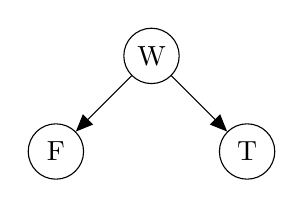
\begin{tikzpicture}
        \node[latent] (W) {W};
        \node[latent, below right=of W] (T) {T};
        \node[latent, below left=of W] (F) {F};
        \edge {W} {F};
        \edge {W} {T};
      \end{tikzpicture}
    \end{subfigure}%
    \begin{subfigure}{0.8\textwidth}
      \centering
      \begin{tabular}[t]{cc}
        \toprule
        $w$ & $\Pr(W = w)$ \\
        \midrule
        1 & 0.5 \\
        0 & 0.5 \\
        \bottomrule
      \end{tabular}
      \begin{tabular}[t]{ccc}
        \toprule
        $w$ & $f$ & $\Pr(F = f \mid W = w)$ \\
        \midrule
        1 & 1 & 0.6 \\
        1 & 0 & 0.4 \\
        0 & 1 & 0.1 \\
        0 & 0 & 0.9 \\
        \bottomrule
      \end{tabular}
      \begin{tabular}[t]{ccc}
        \toprule
        $w$ & $t$ & $\Pr(T = t \mid W = w)$ \\
        \midrule
        1 & $l$ & 0.2 \\
        1 & $m$ & 0.4 \\
        1 & $h$ & 0.4 \\
        0 & $l$ & 0.6 \\
        0 & $m$ & 0.3 \\
        0 & $h$ & 0.1 \\
        \bottomrule
      \end{tabular}
    \end{subfigure}
    \caption{An example Bayesian network with its CPTs}
    \label{fig:example_bn}
  \end{figure}

  The Bayesian network in \cref{fig:example_bn} has
  \begin{align*}
    V &= \{ W, F, T \}, \\
    \mathrm{pa}(W) &= \emptyset, \\
    \mathrm{pa}(F) &= \mathrm{pa}(T) = \{ W \}, \\
    \im W &= \im F = \{ 0, 1 \}, \\
    \im T &= \{ l, m, h \}, \\
    E(W) &= \{ \lambda_{W=1} \}, \\
    E(F) &= \{ \lambda_{F=1} \}, \\
    E(T) &= \{ \lambda_{T=l}, \lambda_{T=m}, \lambda_{T=h} \}, \\
    E^*(W) &= \{ \lambda_{W=1} \}, \\
    E^*(F) &= \{ \lambda_{F=1}, \lambda_{W=1} \}, \\
    E^*(T) &= \{ \lambda_{T=l}, \lambda_{T=m}, \lambda_{T=h}, \lambda_{W=1} \}, \\
    \mathrm{CPT_W} &= 0.5[\lambda_{W=1}]+0.5\overline{[\lambda_{W=1}]} = 0.5 \cdot 1, \\
    \mathrm{CPT_F} &= 0.6[\lambda_{F=1}] \cdot [\lambda_{W=1}] + 0.4[\lambda_{F=0}] \cdot [\lambda_{W=1}] + 0.1[\lambda_{F=1}] \cdot [\lambda_{W=0}] + 0.9[\lambda_{F=0}] \cdot [\lambda_{W=0}] \\
      &= 0.6[\lambda_{F=1}] \cdot [\lambda_{W=1}] + 0.4\overline{[\lambda_{F=1}]} \cdot [\lambda_{W=1}] + 0.1[\lambda_{F=1}] \cdot \overline{[\lambda_{W=1}]} + 0.9\overline{[\lambda_{F=1}]} \cdot \overline{[\lambda_{W=1}]}, \\
    \mathrm{CPT_T} &= ([\lambda_{T=l}] + [\lambda_{T=m}] + [\lambda_{T=h}]) \cdot (\overline{[\lambda_{T=l}]} + \overline{[\lambda_{T=m}]}) \cdot (\overline{[\lambda_{T=l}]} + \overline{[\lambda_{T=h}]}) \cdot (\overline{[\lambda_{T=m}]} + \overline{[\lambda_{T=h}]}) \cdot (\dots),
  \end{align*}
  and can be encoded in a DIMACS-like CNF format as
  \[
    \begin{array}{l r r l l}
      \lambda\sb{T=l} &\lambda\sb{T=m} &\lambda\sb{T=h} & &0 \\
                      &-\lambda\sb{T=l} &-\lambda\sb{T=m} & &0 \\
                      &-\lambda\sb{T=l} &-\lambda\sb{T=h} & &0 \\
                      &-\lambda\sb{T=m} &-\lambda\sb{T=h} & &0 \\
      w &\lambda\sb{W=1} & &0.5 &0.5 \\
      w &\lambda\sb{F=1} &\lambda\sb{W=1} &0.6 &0.4 \\
      w &\lambda\sb{F=1} &-\lambda\sb{W=1} &0.1 &0.9 \\
      w &\lambda\sb{T=l} &\lambda\sb{W=1} &0.2 &1 \\
      w &\lambda\sb{T=m} &\lambda\sb{W=1} &0.4 &1 \\
      w &\lambda\sb{T=h} &\lambda\sb{W=1} &0.4 &1 \\
      w &\lambda\sb{T=l} &\lambda\sb{W=0} &0.6 &1 \\
      w &\lambda\sb{T=m} &\lambda\sb{W=0} &0.3 &1 \\
      w &\lambda\sb{T=h} &\lambda\sb{W=0} &0.1 &1
    \end{array}
  \]
  with each $\lambda$ replaced with a unique positive integer.
\end{example}

The last two numbers are the positive and the negative probabilities,
respectively---sometimes they add to one, and sometimes the negative probability
is one, regardless of the value of the first probability.

\section{Experimental Comparison}

\begin{itemize}
\item We don't compare 'compile times' because our encoding time is linear, so
  we would easily beat everyone else.
\item When the Bayesian network has an evidence file, we compute the probability
  of evidence. Otherwise, let $X$ denote the last-mentioned node in the Bayesian
  network. If $\mathsf{true}$ is a valid value of $X$, we compute the marginal
  probability of $X = \mathsf{true}$. Otherwise, we pick the first value of $X$
  and calculate its marginal probability. This applies to the Grid data set (as
  intended) and also to two instances of Plan Reconstruction and roughly half of
  the instances from 2004-PGM that have empty evidence files.
\item After the experiments are finished, note the processor, memory per thread,
  and add the following acknowledgment.
\item All other encodings are implemented in
  Ace~3.0\footnote{\url{http://reasoning.cs.ucla.edu/ace/}} and should be
  compiled with \texttt{-encodeOnly} (i.e., don't compile the CNF into an AC)
  and \texttt{-noEclause} (i.e., only use standard syntax) flags.
\item Datasets
  \begin{itemize}
  \item binary Bayesian networks from Sang et
    al.\footnote{\url{https://www.cs.rochester.edu/u/kautz/Cachet/}}
    \cite{DBLP:conf/aaai/SangBK05}
    \begin{itemize}
    \item Grid (networks) (ratio 75 means that 75\% of the nodes are
      deterministic),
    \item Plan recognition (problems),
    \item Deterministic quick medical reference (what do the numbers mean? the
      README doesn't say).
    \end{itemize}
  \item Bayesian networks available with Ace
    \begin{itemize}
    \item \texttt{2004-pgm} \cite{DBLP:journals/ijar/ChaviraDJ06} (binary)
    \item \texttt{2005-ijcai} \cite{DBLP:conf/ijcai/ChaviraD05}. The Genie/Smile
      files have their own citation data that I should probably extract. This is
      the only dataset that has some non-binary networks.
    \item \texttt{2006-ijar} \cite{DBLP:journals/ijar/ChaviraDJ06} (binary)
    \end{itemize}
  \end{itemize}
\end{itemize}

\section{Explaining The Performance Benefits}

\begin{itemize}
\item \texttt{d02} has
  \[
    \sum_{X \in V} |\im X| + |\im X|\prod_{Y \in \mathrm{pa}(X)}|\im Y|
  \]
  variables and
  \[
    \sum_{X \in V} 1 + \binom{|\im X|}{2} + |\im X|(2 +
    |\mathrm{pa}(X)|)\prod_{Y \in \mathrm{pa}(X)} |\im Y|
  \]
  clauses (along with one ADD per variable to encode the weights).
\item \texttt{sbk05} is a bit harder to evaluate due to a handful of small
  optimisations in the encoding. Could find an upper bound anyway.
\item \texttt{db20} (my encoding) has
  \[
    \sum_{X \in V} |\im X|
  \]
  variables (less for binary) and
  \[
    \sum_{X \in V} |\im X| + 1 + \binom{|\im X|}{2}
  \]
  ADDs.
\item Let:
  \begin{itemize}
  \item $N = |V|$ (i.e., the number of nodes in the Bayesian network),
  \item $D = \max_{X \in V} |\mathrm{pa}(X)|$ (i.e., the maximum in-degree or
    the number of parents),
  \item $V = \max_{X \in V} |\im X|$ (i.e., the maximum number of values per
    variables).
  \end{itemize}
\item Then my encoding has $\mathcal{O}(NV)$ variables and $\mathcal{O}(NV^2)$
  ADDs while \texttt{d02} has $\mathcal{O}(NV^{D+1})$ variables and
  $\mathcal{O}(NDV^{D+1})$ ADDs.
\end{itemize}

\todo[inline]{Calculate numVariables/numClauses (or the other way around) for
  each instance and plot this ratio vs runtime (for each encoding, or at least
  mine and D02)}

\section{Conclusion and Future Work}

\begin{itemize}
\item Bayesian networks and ADDMC are only particular examples. This should also
  work with Cachet.
\item Extra benefit: one does not need to come up with a way to turn some
  probability distribution to into a fully independent one.
\item Important future work: replacing ADDs with
  AADDs\footnote{\url{https://github.com/ssanner/dd-inference}}
  \cite{DBLP:conf/ijcai/SannerM05} is likely to bring performance benefits.
  Other extensions:
  \begin{itemize}
  \item FOADDs can represent first order statements;
  \item XADDs can replace WMI for continuous variables;
  \item ADDs with intervals can do approximations.
  \end{itemize}
\item Filtering out ADDs that have nothing to do with the answer helps
  tremendously, but I'm purposefully not doing that. Perhaps a heuristic could
  do the same thing?
\item Encodings for everything else
  \begin{itemize}
  \item probabilistic programs \cite{DBLP:journals/corr/abs-2005-09089}
  \item ProbLog \cite{DBLP:conf/uai/FierensBTGR11}
    \begin{itemize}
    \item For the ProbLog to WMC conversion, check out this guy:
      \url{https://users.ics.aalto.fi/ttj/}.
    \item proof-based \cite{DBLP:conf/iclp/MantadelisJ10}
    \item rule-based \cite{DBLP:conf/ecai/Janhunen04}
    \item For ground ProbLog, we can encode a program
\begin{verbatim}
p :: a :- b
q :: a :- c
\end{verbatim}
      into $P(a \mid b)=p$, $P(a \mid c)=q$ instead of having clauses $b
      \Rightarrow a$, $c \Rightarrow a$. Some logical structure is likely to
      remain.
    \end{itemize}
  \end{itemize}
\item Bayesian networks are often solved in a compile once, query many times
  fashion. This can be achieved using ADDMC by selecting a subset $S$ of
  variable we may want to query over and running ADDMC while excluding $S$ from
  variable elimination/projection/$\exists$.
\item More references
  \begin{itemize}
  \item Measures on/in Boolean algebras: Horn and Tarski
    \cite{horn1948measures}, Jech \cite{jech2017measures}
  \item On Boolean algebras and their role in analysis \cite{winkowska1996boolean}
  \item Infinite domains
    \begin{itemize}
    \item Markov Logic in Infinite Domains (Singla and Domingos)
      \cite{DBLP:conf/uai/SinglaD07}
    \item Objective Bayesian probabilistic logic (Williamson)
      \cite{DBLP:journals/jal/Williamson08}
    \item Unifying Logic and Probability (Russell)
      \cite{DBLP:journals/cacm/Russell15}
    \end{itemize}
  \item Logical induction \cite{DBLP:journals/eccc/GarrabrantBCST16}
  \item Quantum probabilistic logic programming \cite{balu2015quantum}
  \item WMC
    \begin{itemize}
    \item algebraic model counting \cite{DBLP:journals/japll/KimmigBR17}
    \item Explanation-Based Approximate Weighted Model Counting for
      Probabilistic Logics \cite{DBLP:conf/aaai/RenkensKBR14}
    \item OUWMC \cite{DBLP:conf/aaai/Belle17}
    \item Formula-Based Probabilistic Inference \cite{DBLP:conf/uai/GogateD10}
    \item Parallel Probabilistic Inference by WMC \cite{DBLP:conf/pgm/DalLL18}
    \item Semiring Programming \cite{DBLP:journals/corr/BelleR16}
    \item theoretical extension: WMC beyond two-variable logic
      \cite{DBLP:conf/lics/KuusistoL18}
    \item from weighted to unweighted model counting
      \cite{DBLP:conf/ijcai/ChakrabortyFMV15}
    \item theory behind WMC algorithms: solving \#\SAT{} and Bayesian inference
      with backtracking search \cite{DBLP:journals/jair/BacchusDP09}
    \end{itemize}
  \end{itemize}
\end{itemize}

\paragraph{Acknowledgements.} This work has made use of the resources provided
by the Edinburgh Compute and Data Facility (ECDF)
(\url{http://www.ecdf.ed.ac.uk/}).

\bibliographystyle{plain}
\bibliography{paper}

\end{document}
